\documentclass{article}
\usepackage{graphicx} % Required for inserting images
\usepackage{pgffor}
\usepackage{listings}
\usepackage{xcolor}
\usepackage{hyperref}
\usepackage{amsmath}
\usepackage{mathtools}
\usepackage{enumitem}
\usepackage{pifont}
\usepackage{amssymb}
\usepackage{array}
\usepackage{multirow}
\usepackage{makecell}
\usepackage{fancyhdr}
\usepackage{colortbl}
\usepackage{multicol}
\usepackage{longtable}
\usepackage{cite}
\usepackage{float}
\usepackage{tabularx}
\usepackage[vietnamese, english]{babel}
\usepackage[a4paper, total={6in, 8in}, margin=1in]{geometry}
\usepackage{styles/standard}

\allowdisplaybreaks
\setlength{\parindent}{0pt}
\setlength{\headheight}{40pt}
\setlength{\parskip}{0.3em}
\renewcommand{\arraystretch}{1.6}

\title{ \normalsize \textsc{}
		\\ [2.0cm]
        % \HRule{1.5pt} \\
        \begin{tabular}{c@{\hskip 2cm}c}
            
\includegraphics[width=0.3\textwidth]{styles/logoHCMUS.png}
            &
            
\includegraphics[width=0.3\textwidth]{styles/logoAPCS.png}
        \end{tabular}
        \vspace{2em} \\
        \vspace{6pt}
        \LARGE \textbf{\uppercase{CS420 -- Artificial Intelligence}} \\
		\LARGE \textbf{Project 2 -- Decision Tree} \\
        \Large \textbf{Report} \\
        \vspace*{13\baselineskip}
}
\author{
    VNUHCM-UNIVERSITY OF SCIENCE \\
    \today
}
\date{}

\pagestyle{fancy}
\fancyhead[L]{\textbf{Project 2 -- Decision Tree}}
\fancyhead[R]{
\includegraphics[width=1.25cm]{styles/logoAPCS.png}}

\begin{document}

\maketitle
\thispagestyle{empty}
\newpage

\selectlanguage{vietnamese}
\thispagestyle{empty}
\section*{Student Information}
\begin{table}[h]
    \centering
    \begin{tabular}{|c|c|}
        \hline
        \textbf{Full Name} & \textbf{Student ID} \\ \hline 
        Vòng Vĩnh Toàn & 22125108 \\ \hline
        Nguyễn Hoàng Phúc & 22125077\\ \hline
        Huỳnh Hà Phương Linh & 22125049\\ \hline
        Huỳnh Đăng Khoa & 22125038 \\ 
        \hline
    \end{tabular}
\end{table}
\selectlanguage{english}
\newpage

\tableofcontents
\thispagestyle{empty}
\newpage

\setcounter{page}{1}
\Section{Introduction}

The Decision Tree algorithm is a supervised learning algorithm that can be used for both classification and regression tasks. The algorithm works by recursively splitting the dataset into subsets based on the most discriminative features. The splitting process continues until the tree reaches a maximum depth or the number of samples in a node falls below a certain threshold. The Decision Tree algorithm is simple to understand and interpret, making it an excellent choice for tasks that require transparency and interpretability.

In this project, we implement the Decision Tree algorithm using Python and the \texttt{scikit-learn} library. We evaluate the algorithm's performance on three different datasets from the UCI Machine Learning Repository. The datasets are as follows:
\begin{enumerate}
    \item The UCI Breast Cancer Wisconsin dataset \cite{breast_cancer_wisconsin}
    \item The UCI Wine Quality dataset \cite{wine_quality}
    \item The UCI User Knowledge Modeling dataset \cite{user_knowledge_modeling}
\end{enumerate}

Note that \textbf{all figures and tables} in this report are in the \textbf{vector image format} for better readability and quality as the reader zooms in since the illustrations can be too complex to be displayed.

\newpage
\setcounter{section}{1}
\Section{Dataset 1: The UCI Breast Cancer Wisconsin}

In this Section, we will present the classification results of the first dataset that we used in our project, which is the UCI Breast Cancer Wisconsin dataset \cite{breast_cancer_wisconsin}.

The dataset contains features computed from a digitized image of a fine needle aspirate (FNA) of a breast mass. These features describe characteristics of the cell nuclei present in the image. A sample of such images can be found at \url{http://www.cs.wisc.edu/~street/images/}.

\subsubsection*{Dataset Characteristics}
\begin{itemize}
    \item \textbf{Type:} Multivariate
    \item \textbf{Subject Area:} Health and Medicine
    \item \textbf{Associated Task:} Classification
    \item \textbf{Feature Type:} Real-valued
    \item \textbf{Number of Instances:} 569
    \item \textbf{Number of Features:} 30
    \item \textbf{Missing Values:} No
\end{itemize}

\subsubsection*{Dataset Insights}
\begin{itemize}
    \item \textbf{Source:} Digitized images of fine needle aspirates (FNA) of breast masses.
    \item \textbf{Objective:} Classify tumors as malignant (M) or benign (B).
    \item \textbf{Methodology:} Features were computed using image analysis techniques to describe characteristics of cell nuclei.
    \item \textbf{Additional Details:}
    \begin{itemize}
        \item Separating planes were determined using the Multisurface Method-Tree (MSM-T).
        \item Feature selection involved exhaustive searches in feature and plane spaces.
    \end{itemize}
\end{itemize}

\subsubsection*{Feature Description}
\begin{itemize}
    \item \textbf{Input Variables:} Ten real-valued features computed for each cell nucleus:
    \begin{enumerate}
        \item \textbf{Radius:} Mean distance from the center to the perimeter.
        \item \textbf{Texture:} Standard deviation of gray-scale values.
        \item \textbf{Perimeter:} Measurement of the contour length.
        \item \textbf{Area:} Size of the cell nucleus.
        \item \textbf{Smoothness:} Local variation in radius lengths.
        \item \textbf{Compactness:} Computed as $(\text{perimeter}^2 / \text{area}) - 1.0$.
        \item \textbf{Concavity:} Severity of concave portions of the contour.
        \item \textbf{Concave Points:} Number of concave portions of the contour.
        \item \textbf{Symmetry:} Symmetry of the cell nucleus.
        \item \textbf{Fractal Dimension:} Approximation of the contour's fractal nature.
    \end{enumerate}
    \item \textbf{Output Variable:}
    \begin{itemize}
        \item Diagnosis: Binary classification where M = malignant and B = benign.
    \end{itemize}
\end{itemize}
\subsection{Data preparation}

\subsubsection{Import the dataset}

The \href{https://archive.ics.uci.edu/}{UC Irvine Machine Learning Repository} allows for direct dataset import in Python using the \texttt{ucimlrepo} package. The package is included in the \texttt{requirements.txt} file. The following code demonstrates how to import the Breast Cancer Wisconsin (id = 17) dataset using the \texttt{fetch\_ucirepo} function:

\lstset{style=code}
\begin{lstlisting}[language=Python]
from ucimlrepo import fetch_ucirepo 

breast_cancer_wisconsin_diagnostic = fetch_ucirepo(id=17) 
    
X = breast_cancer_wisconsin_diagnostic.data.features 
y = breast_cancer_wisconsin_diagnostic.data.targets 
\end{lstlisting}

\subsubsection{Splitting the dataset}

The dataset is split into training and testing sets using the \texttt{train\_test\_split} function from the \texttt{sklearn} library. 
The dataset is splitted into 4 sets of different test sizes: 60\%, 40\%, 20\%, and 10\% of the dataset in stratified fashion, using the random state of 22125 to ensure reproducibility.

\begin{figure}[H]
    \centering
    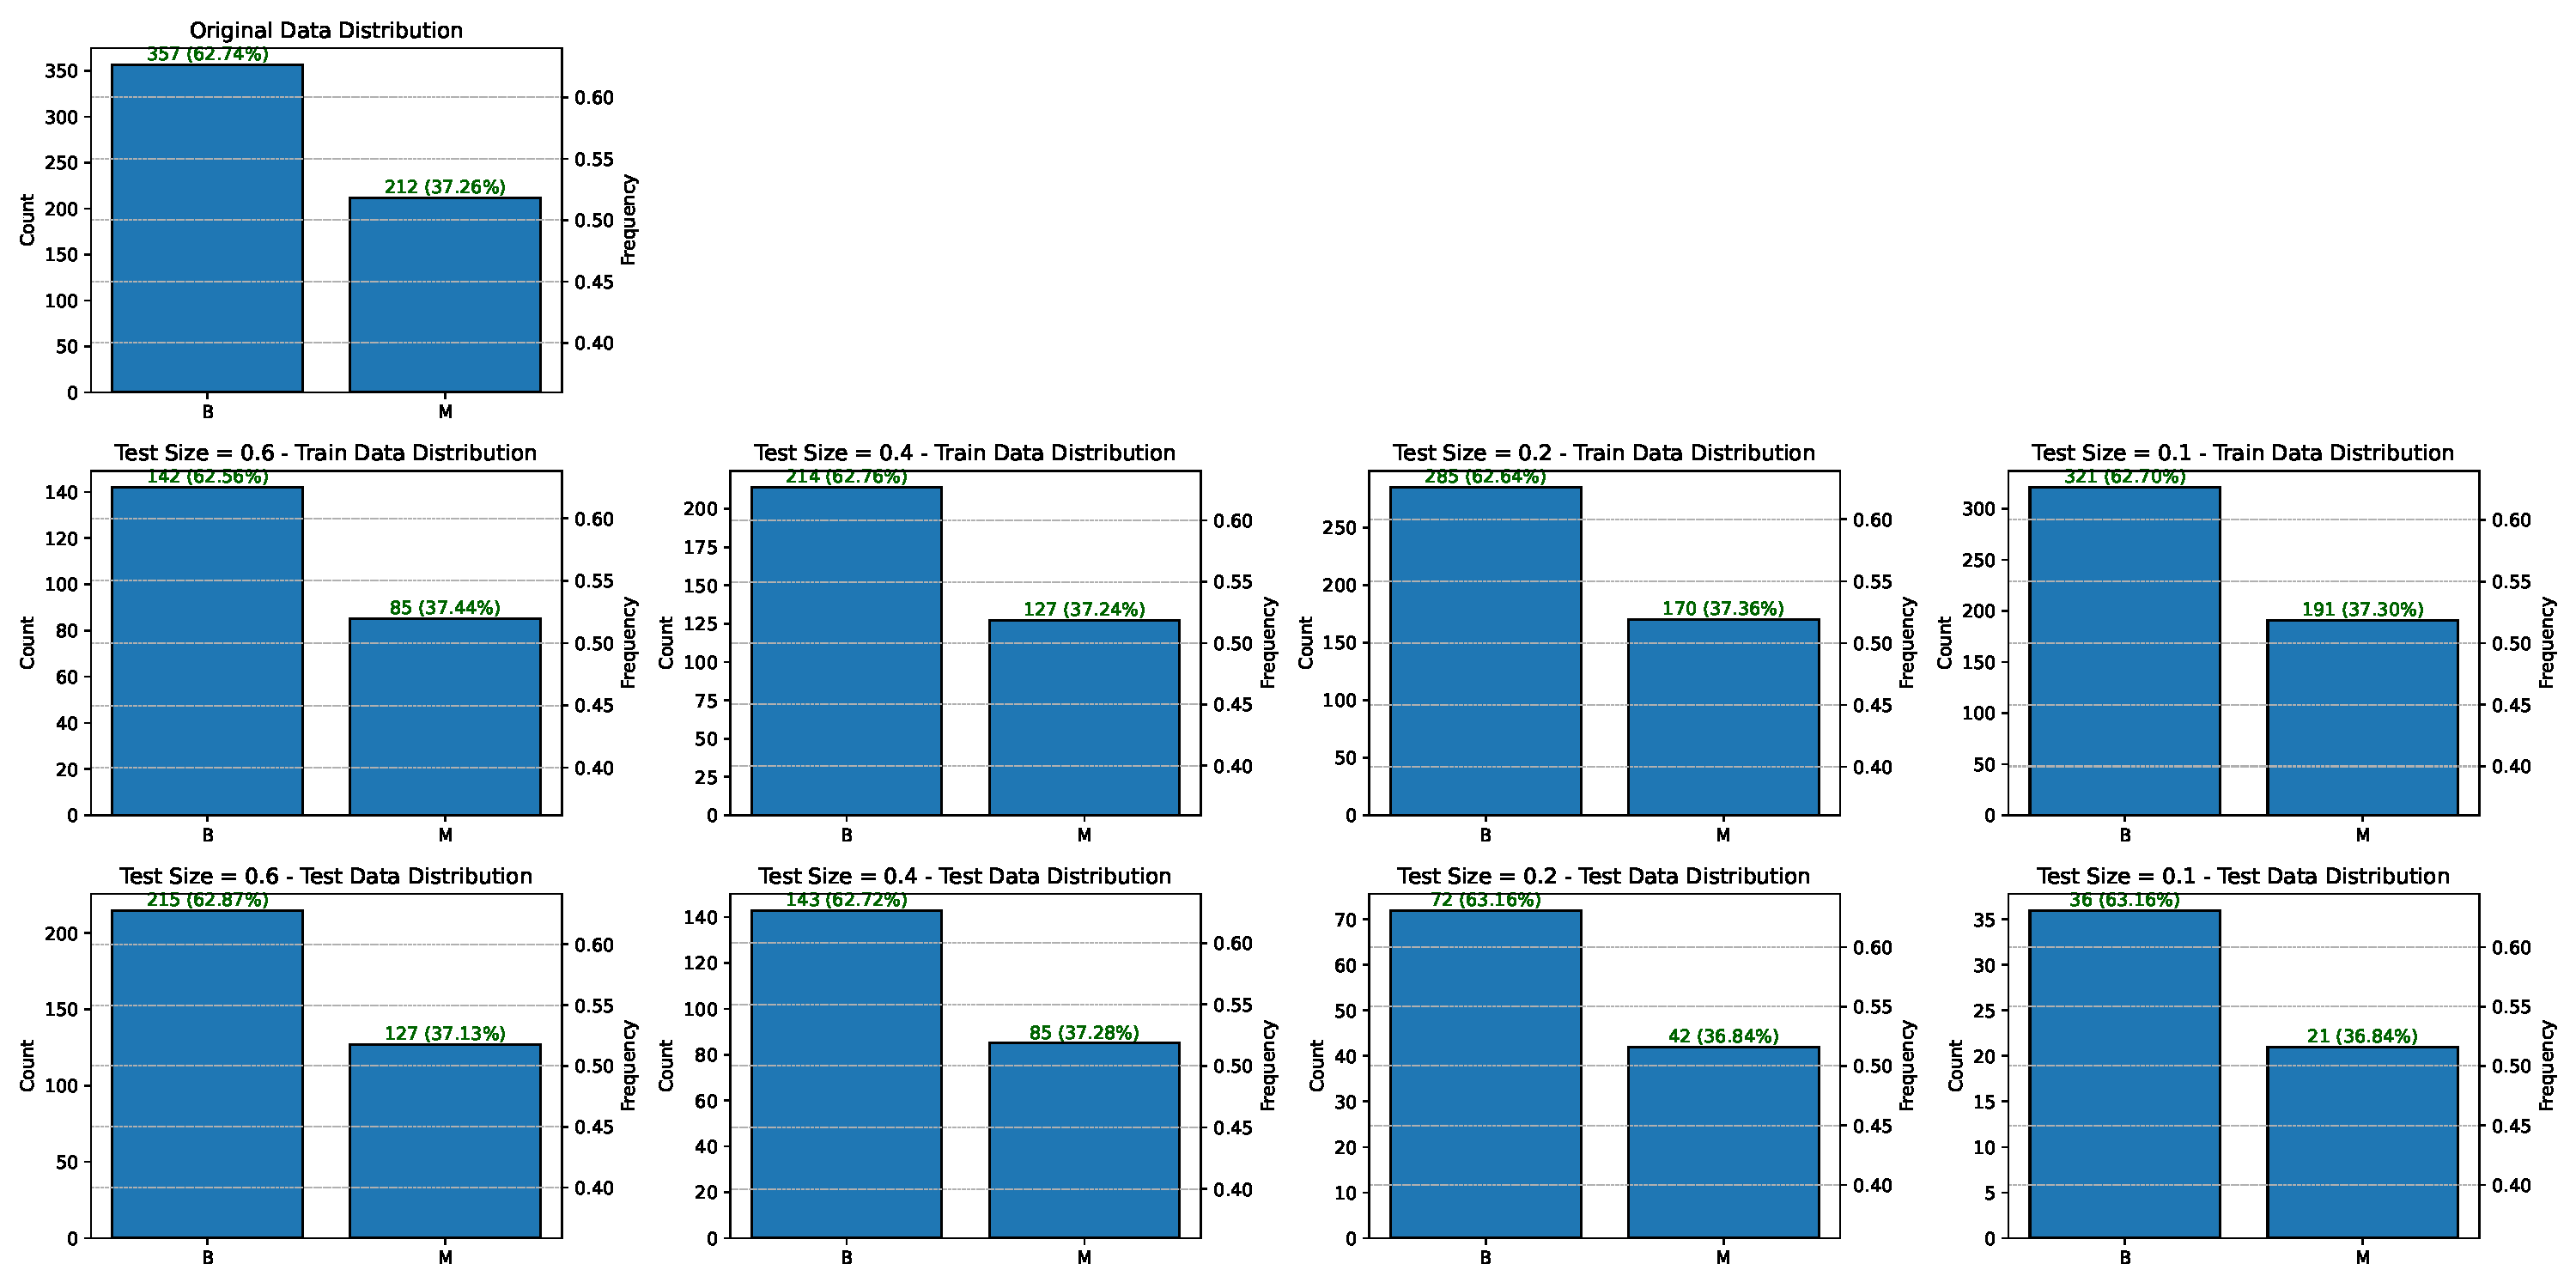
\includegraphics[width=\textwidth]{figures/breast_cancer_wisconsin_split.pdf}
    \caption{Breast Cancer Wisconsin dataset split}
    \label{fig:breast_cancer_wisconsin_split}
\end{figure}

As shown in figure \ref{fig:breast_cancer_wisconsin_split}, the distribution of the target class is preserved in all splits.

\subsection{Decision Tree classifier implementation}

Decision Tree classifiers are implemented using the \texttt{DecisionTreeClassifier} class from the \texttt{sklearn} library. 
To ensure reproducibility, the random state is set to 22125. 
We use the Entropy (information gain) criterion to split the nodes and set the maximum depth of the tree to None to allow the tree to grow until all leaves are pure.

\begin{figure}[H]
    \centering
    \includegraphics[width=\textwidth]{figures/breast_cancer_wisconsin_decision_trees.pdf}
    \caption{Breast Cancer Wisconsin dataset Decision Trees with different test sizes}
    \label{fig:breast_cancer_wisconsin_decision_trees}
\end{figure}

The Decision Trees are visualized in figure \ref{fig:breast_cancer_wisconsin_decision_trees}. The trees grow deeper as the test size decreases, indicating that the model is more complex and overfits the training data when the test size is small.

The first node of the Decision Tree splits the dataset based on different features:
\begin{itemize}
    \item Decision tree of test size 60\% chooses the feature \texttt{concave\_points3} to split the dataset.
    \item Decision tree of test size 40\% and 20\% chooses the feature \texttt{area3} to split the dataset.
    \item Decision tree of test size 10\% chooses the feature \texttt{perimeter3} to split the dataset.
\end{itemize}

Despite the differences in the splitting features, the first node's entropy is approximately 0.953 in all Decision Trees, indicating that the first split is not very informative. However, the Decision Tree classifier effectively splits the dataset into pure leaves with high information gain.

\subsection{Performance evaluation}

\subsubsection{Classification report}

The classification report provides a comprehensive evaluation of the Decision Tree classifier's performance using the \texttt{classification\_report} function from the \texttt{sklearn.metrics} module. The report includes the following metrics:
\begin{itemize}
    \item \textbf{Precision:} The ratio of true positive samples to the sum of true positive and false positive samples.
    \item \textbf{Recall:} The ratio of true positive samples to the sum of true positive and false negative samples.
    \item \textbf{F1-score:} The harmonic mean of precision and recall.
    \item \textbf{Support:} The number of samples in each class.
\end{itemize}

\textbf{Classification Report for Test Size = 0.6}

\begin{tabular}{lcccccc}
\hline
 & \textbf{Precision} & \textbf{Recall} & \textbf{F1-score} & \textbf{Support} \\
\hline
B & 0.94 & 0.94 & 0.94 & 215 \\
M & 0.90 & 0.89 & 0.89 & 127 \\
\hline
\textbf{Accuracy} & & & 0.92 & 342 \\
\textbf{Macro avg} & 0.92 & 0.91 & 0.92 & 342 \\
\textbf{Weighted avg} & 0.92 & 0.92 & 0.92 & 342 \\
\hline
\end{tabular}

\vspace{2em}

\textbf{Classification Report for Test Size = 0.4}

\begin{tabular}{lcccccc}
\hline
 & \textbf{Precision} & \textbf{Recall} & \textbf{F1-score} & \textbf{Support} \\
\hline
B & 0.94 & 0.92 & 0.93 & 143 \\
M & 0.87 & 0.89 & 0.88 & 85 \\
\hline
\textbf{Accuracy} & & & 0.91 & 228 \\
\textbf{Macro avg} & 0.91 & 0.91 & 0.90 & 228 \\
\textbf{Weighted avg} & 0.91 & 0.91 & 0.91 & 228 \\
\hline
\end{tabular}

\vspace{2em}

\textbf{Classification Report for Test Size = 0.2}

\begin{tabular}{lcccccc}
\hline
 & \textbf{Precision} & \textbf{Recall} & \textbf{F1-score} & \textbf{Support} \\
\hline
B & 0.95 & 0.88 & 0.91 & 72 \\
M & 0.81 & 0.93 & 0.87 & 42 \\
\hline
\textbf{Accuracy} & & & 0.89 & 114 \\
\textbf{Macro avg} & 0.89 & 0.90 & 0.88 & 114 \\
\textbf{Weighted avg} & 0.90 & 0.89 & 0.90 & 114 \\
\hline
\end{tabular}

\vspace{100em}

\textbf{Classification Report for Test Size = 0.1}

\begin{tabular}{lcccccc}
\hline
 & \textbf{Precision} & \textbf{Recall} & \textbf{F1-score} & \textbf{Support} \\
\hline
B & 0.97 & 0.92 & 0.94 & 36 \\
M & 0.87 & 0.95 & 0.91 & 21 \\
\hline
\textbf{Accuracy} & & & 0.93 & 57 \\
\textbf{Macro avg} & 0.93 & 0.93 & 0.92 & 57 \\
\textbf{Weighted avg} & 0.93 & 0.93 & 0.93 & 57 \\
\hline
\end{tabular}

The classification reports show that the Decision Tree classifier performs well on the Breast Cancer Wisconsin dataset, achieving an accuracy of 92\% for the test size of 60\%, 91\% for the test size of 40\%, 89\% for the test size of 20\%, and 93\% for the test size of 10\%. The classifier has high precision, recall, and F1-score for both classes, indicating that it effectively distinguishes between malignant and benign samples.

Prediction performance is better for the benign class, with higher precision, recall, and F1-scores across all test sizes, likely due to the dataset's imbalance favoring benign samples.
\subsubsection{Confusion matrix}

The confusion matrix provides a visual representation of the Decision Tree classifier's performance using the \texttt{confusion\_matrix} function from the \texttt{sklearn.metrics} module. The matrix shows the number of true positive, false positive, true negative, and false negative samples for each class.

\begin{figure}[H]
    \centering
    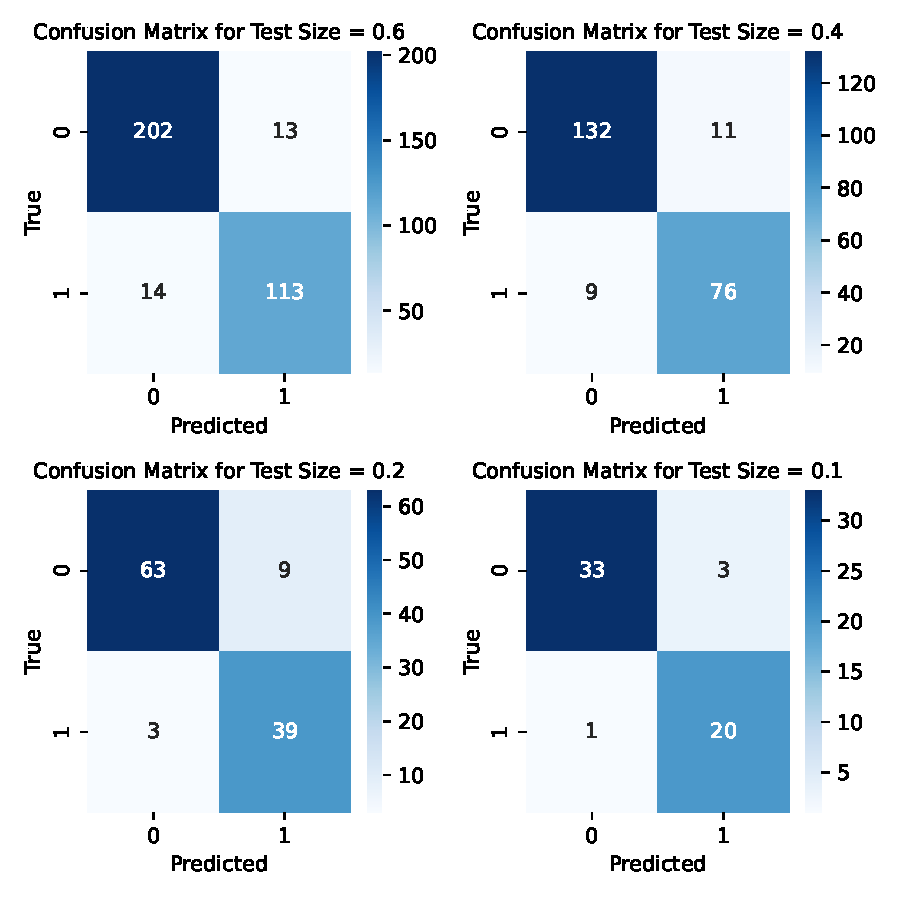
\includegraphics[width=.7\textwidth]{figures/breast_cancer_wisconsin_confusion_matrices.pdf}
    \caption{Breast Cancer Wisconsin dataset Confusion Matrices with different test sizes}
    \label{fig:breast_cancer_wisconsin_confusion_matrices}
\end{figure}
% Confusion Matrix for Test Size = 0.6:
% [[202  13]
%  [ 14 113]]
% Confusion Matrix for Test Size = 0.4:
% [[132  11]
%  [  9  76]]
% Confusion Matrix for Test Size = 0.2:
% [[63  9]
%  [ 3 39]]
% Confusion Matrix for Test Size = 0.1:
% [[33  3]
%  [ 1 20]]

The confusion matrices in figure \ref{fig:breast_cancer_wisconsin_confusion_matrices} show that the Decision Tree classifier correctly classifies most samples in the Breast Cancer Wisconsin dataset. The number of false positive and false negative samples is low, indicating that the classifier has high precision and recall for both classes.

\subsection{Depth vs Accuracy evaluation}

The Decision Tree classifier's performance is evaluated by varying the maximum depth of the tree. The accuracy of the classifier is computed for different maximum depths using the \texttt{accuracy\_score} function from the \texttt{sklearn.metrics} module for the Decision Tree classifier with a test size of 20\%.

\begin{table}[H]
    \centering
    \begin{tabular}{|l|c|c|c|c|c|c|c|}
        \hline
        \textbf{\texttt{max\_depth}} & None & 2 & 3 & 4 & 5 & 6 & 7 \\ \hline
        \textbf{Accuracy} & 0.89 & 0.89 & 0.93 & 0.89 & 0.87 & 0.89 & 0.89 \\ \hline
    \end{tabular}
    \caption{Breast Cancer Wisconsin dataset Depth vs Accuracy}
    \label{tab:breast_cancer_wisconsin_depth_vs_accuracy}
\end{table}

The table \ref{tab:breast_cancer_wisconsin_depth_vs_accuracy} shows that the Decision Tree classifier achieves the highest accuracy on the test data when the maximum depth of the tree is 3. The accuracy decreases as the maximum depth increases, indicating that the model overfits the training data when the tree is too deep.

\begin{figure}[H]
    \centering
    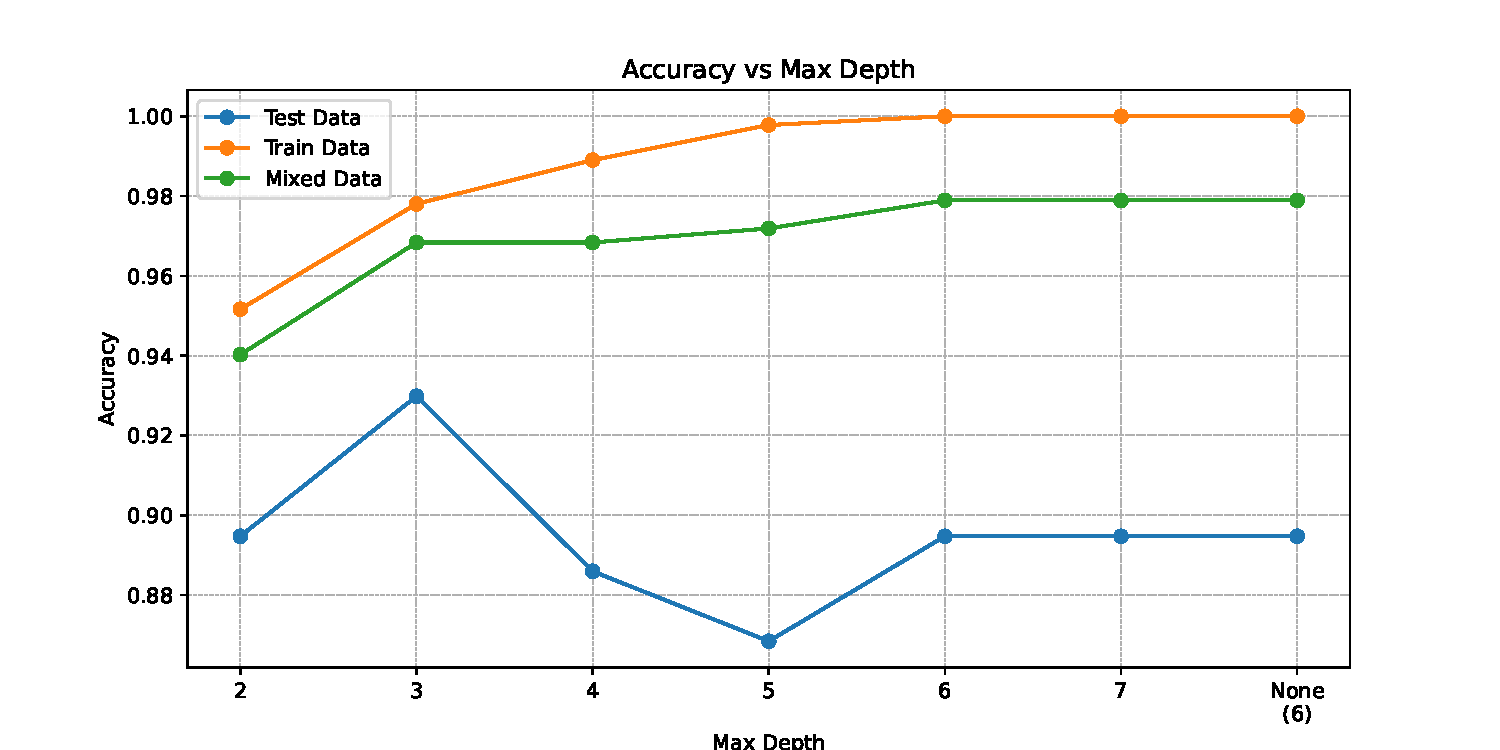
\includegraphics[width=\textwidth]{figures/breast_cancer_wisconsin_accuracy_vs_max_depth.pdf}
    \caption{Breast Cancer Wisconsin dataset Depth vs Accuracy}
    \label{fig:breast_cancer_wisconsin_depth_vs_accuracy}
\end{figure}

The plot in figure \ref{fig:breast_cancer_wisconsin_depth_vs_accuracy} supports the findings in table \ref{tab:breast_cancer_wisconsin_depth_vs_accuracy}.


\newpage
\setcounter{section}{2}
\setcounter{subsection}{0}
\Section{Dataset 2: The Wine Quality}

In this Section, we will present the classification results of the first dataset that we used in our project, which is the UCI Wine Quality dataset \cite{wine_quality}.

The Wine Quality dataset contains data related to red and white variants of the Portuguese "Vinho Verde" wine. The dataset includes physicochemical input variables (e.g., acidity, sugar content, alcohol) and an output variable representing the wine quality. Detailed information about the wine can be found at \url{http://www.vinhoverde.pt/en/} or in the reference by Cortez et al. (2009). 

\subsubsection*{Dataset Characteristics}
\begin{itemize}
    \item \textbf{Type:} Multivariate
    \item \textbf{Subject Area:} Business
    \item \textbf{Associated Tasks:} Classification, Regression
    \item \textbf{Feature Type:} Real
    \item \textbf{Number of Instances:} 4898
    \item \textbf{Number of Features:} 11
    \item \textbf{Missing Values:} No
\end{itemize}

\subsubsection*{Dataset Insights}
\begin{itemize}
    \item \textbf{Data source:} The dataset is derived from physicochemical and sensory tests. No information is provided about grape types, wine brand, or pricing due to privacy and logistical constraints.
    \item \textbf{Task type:} The dataset can be used for both classification and regression tasks. In this project, we focus on the classification task by grouping wine quality into broader categories.
    \item \textbf{Class imbalance:} The dataset is imbalanced, with more samples representing average-quality wines than excellent or poor-quality ones.
    \item \textbf{Feature selection:} Some input variables may not be relevant, making this dataset suitable for testing feature selection methods.
\end{itemize}

\subsubsection*{Feature Description}
\begin{itemize}
    \item \textbf{Input Variables:}
    \begin{enumerate}
        \item Fixed acidity
        \item Volatile acidity
        \item Citric acid
        \item Residual sugar
        \item Chlorides
        \item Free sulfur dioxide
        \item Total sulfur dioxide
        \item Density
        \item pH
        \item Sulphates
        \item Alcohol
    \end{enumerate}
    \item \textbf{Output Variable:}
    \begin{itemize}
        \item Quality: A score between 0 and 10, categorized into three broader groups for analysis:
        \begin{enumerate}
            \item Low quality: Classes 0-4
            \item Standard quality: Classes 5-6
            \item High quality: Classes 7-10
        \end{enumerate}
    \end{itemize}
\end{itemize}

\subsection{Data preparation}

\subsubsection{Import the dataset}

The \href{https://archive.ics.uci.edu/}{UC Irvine Machine Learning Repository} allows for direct dataset import in Python using the \texttt{ucimlrepo} package. The package is included in the \texttt{requirements.txt} file. The following code demonstrates how to import the Wine Quality (id = 186) dataset using the \texttt{fetch\_ucirepo} function:

\lstset{style=code}
\begin{lstlisting}[language=Python]
from ucimlrepo import fetch_ucirepo 

breast_cancer_wisconsin_diagnostic = fetch_ucirepo(id=186) 
    
X = breast_cancer_wisconsin_diagnostic.data.features 
y = breast_cancer_wisconsin_diagnostic.data.targets 
\end{lstlisting}

\subsubsection{Splitting the dataset}

The dataset is split into training and testing sets using the \texttt{train\_test\_split} function from the \texttt{sklearn} library. 
The dataset is splitted into 4 sets of different test sizes: 60\%, 40\%, 20\%, and 10\% of the dataset in stratified fashion, using the random state of 22125 to ensure reproducibility.

\begin{figure}[H]
    \centering
    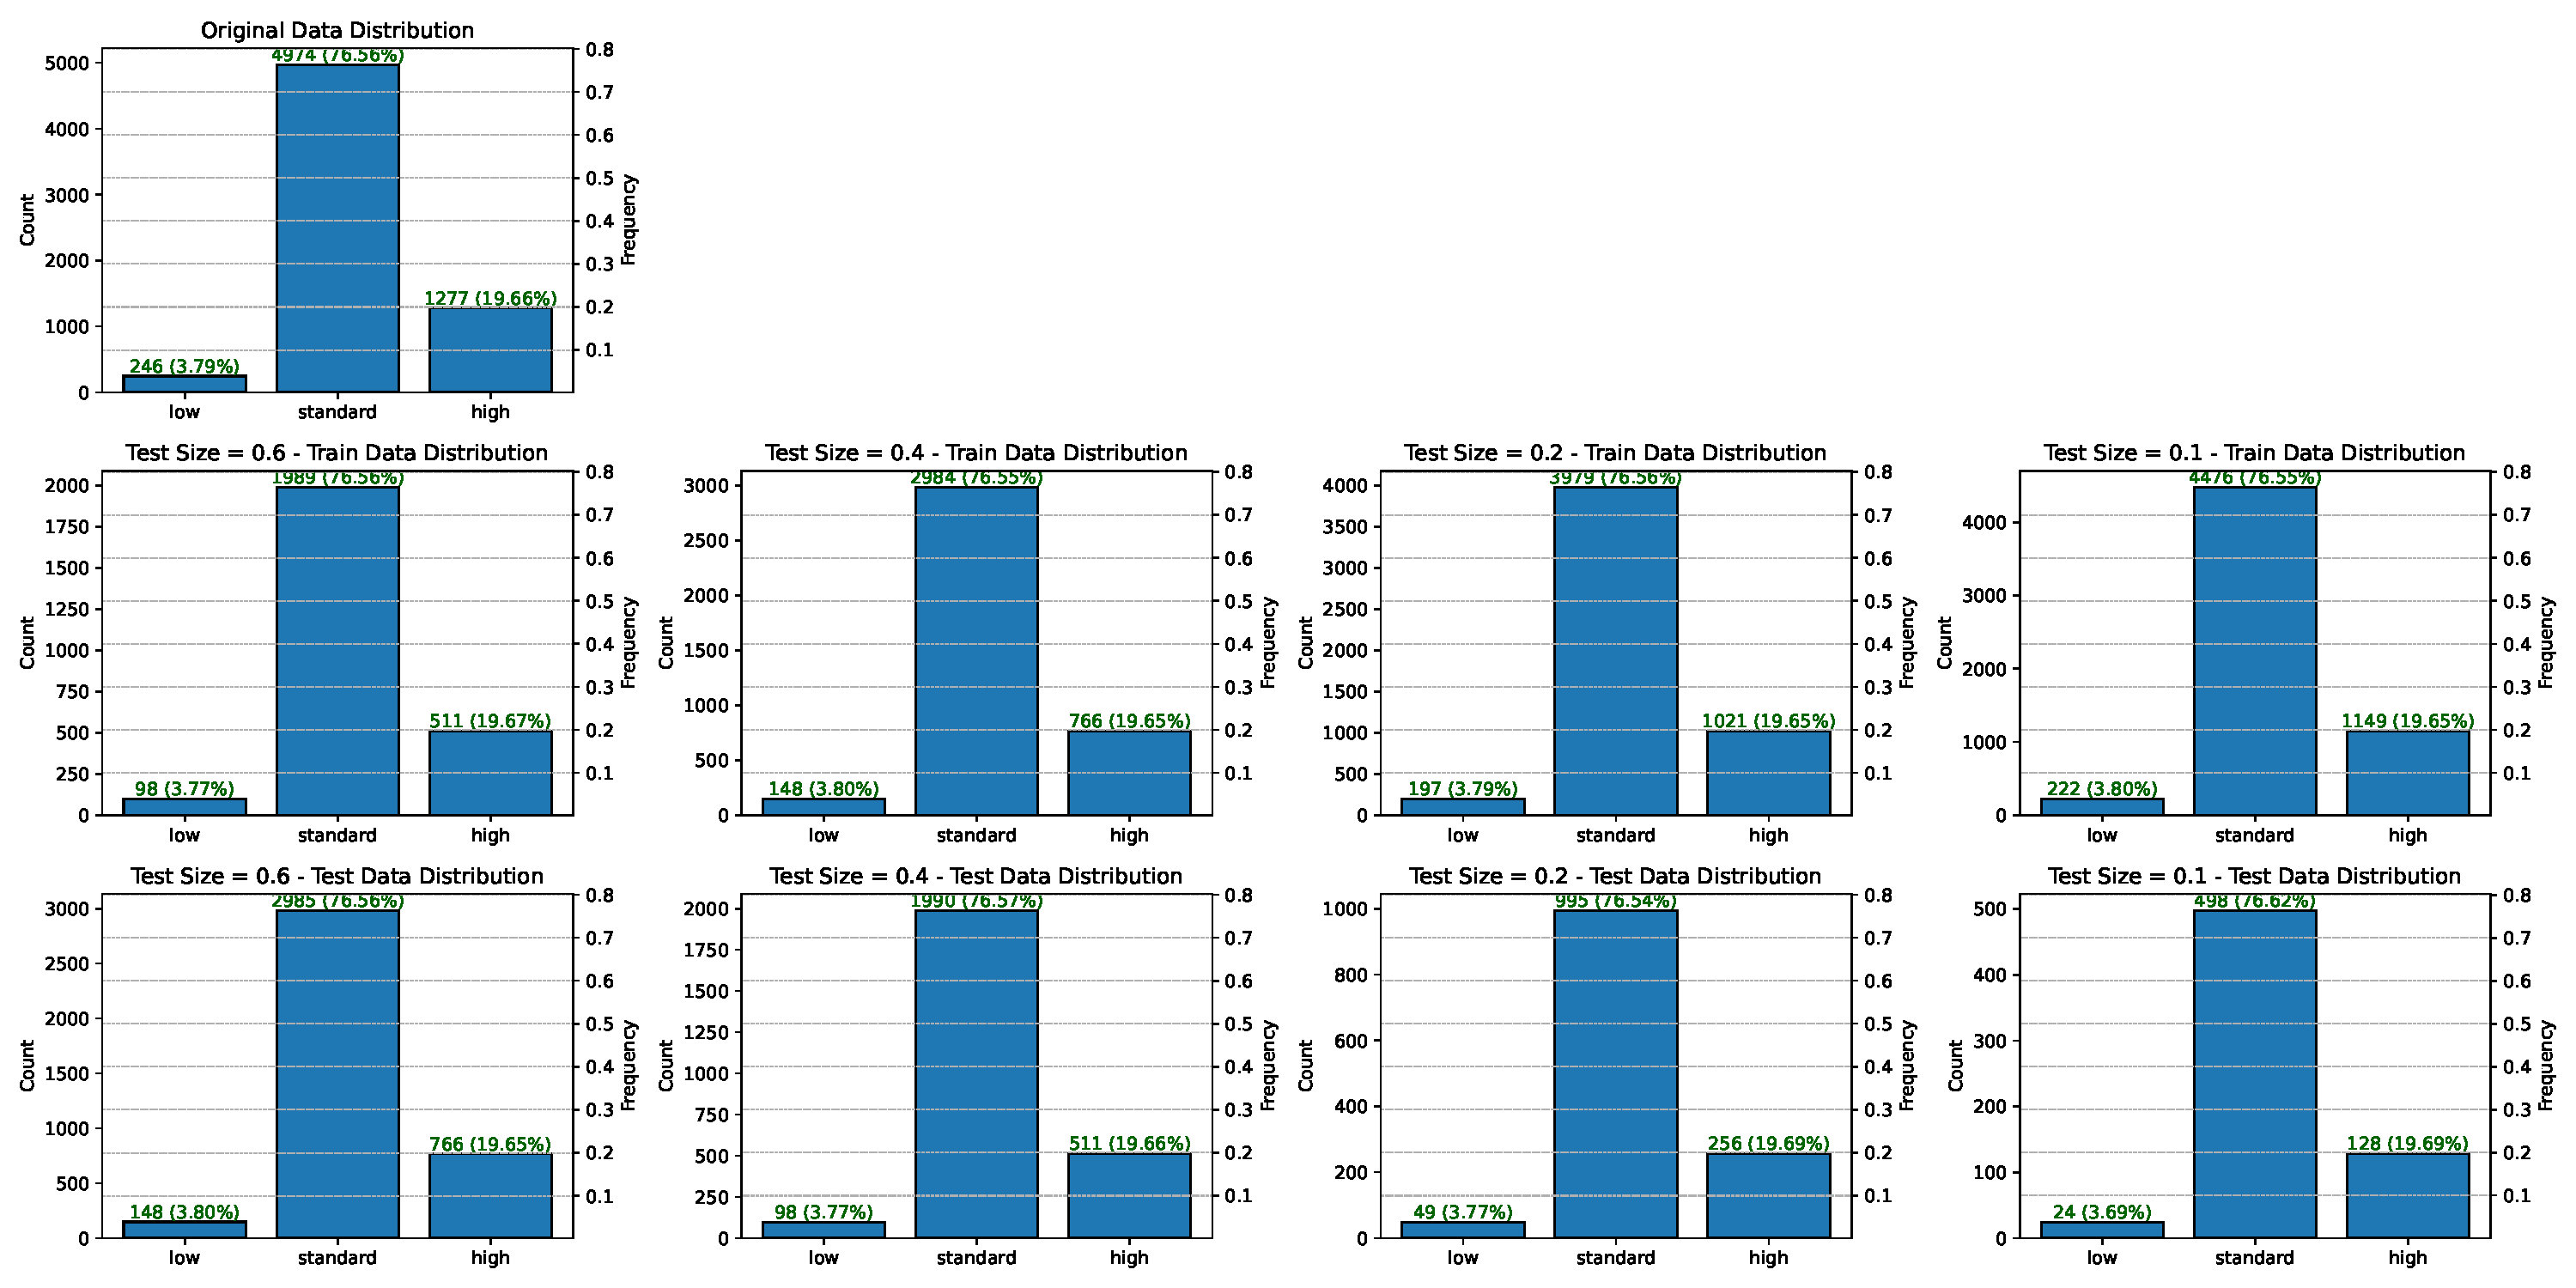
\includegraphics[width=\textwidth]{figures/wine_quality_split.pdf}
    \caption{Breast Cancer Wisconsin dataset split}
    \label{fig:wine_quality_split}
\end{figure}

As shown in figure \ref{fig:wine_quality_split}, the distribution of the target class is preserved in all splits.

\subsection{Decision Tree classifier implementation}

Decision Tree classifiers are implemented using the \texttt{DecisionTreeClassifier} class from the \texttt{sklearn} library. 
To ensure reproducibility, the random state is set to 22125. 
We use the Entropy (information gain) criterion to split the nodes and set the maximum depth of the tree to None to allow the tree to grow until all leaves are pure.

\begin{figure}[H]
    \centering
    \includegraphics[width=\textwidth]{figures/breast_cancer_wisconsin_decision_trees.pdf}
    \caption{Wine Quality dataset Decision Trees with different test sizes}
    \label{fig:wine_quality_decision_trees}
\end{figure}

The Decision Trees are visualized in figure \ref{fig:wine_quality_decision_trees}. 
The depths of the trees for the test sizes 60\%, 40\%, 20\%, and 10\% are 24, 23, 22, and 26 respectively. This indicates that the model complexity does not consistently increase or decrease with the test size.

The first node of the Decision Tree agrees on the feature \texttt{alcohol} to split the dataset for all test sizes. This feature is likely the most discriminative for classifying the wine quality in the dataset.

The first node's entropy is approximately 0.935 in all Decision Trees, indicating that the first split is not very informative. However, the Decision Tree classifier effectively splits the dataset into pure leaves with high information gain.

\subsection{Performance evaluation}

\subsubsection{Classification report}

The classification report provides a comprehensive evaluation of the Decision Tree classifier's performance using the \texttt{classification\_report} function from the \texttt{sklearn.metrics} module. The report includes the following metrics:
\begin{itemize}
    \item \textbf{Precision:} The ratio of true positive samples to the sum of true positive and false positive samples.
    \item \textbf{Recall:} The ratio of true positive samples to the sum of true positive and false negative samples.
    \item \textbf{F1-score:} The harmonic mean of precision and recall.
    \item \textbf{Support:} The number of samples in each class.
\end{itemize}

\textbf{Classification Report for Test Size = 0.6}

\begin{tabular}{lcccccc}
\hline
 & \textbf{Precision} & \textbf{Recall} & \textbf{F1-score} & \textbf{Support} \\
\hline
Low & 0.18 & 0.16 & 0.17 & 148 \\
Standard & 0.85 & 0.85 & 0.85 & 2985 \\
High & 0.53 & 0.55 & 0.54 & 766 \\
\hline
\textbf{Accuracy} & & & 0.76 & 3899 \\
\textbf{Macro avg} & 0.52 & 0.52 & 0.52 & 3899 \\
\textbf{Weighted avg} & 0.76 & 0.76 & 0.76 & 3899 \\
\hline
\end{tabular}

\vspace{2em}

\textbf{Classification Report for Test Size = 0.4}

\begin{tabular}{lcccccc}
\hline
 & \textbf{Precision} & \textbf{Recall} & \textbf{F1-score} & \textbf{Support} \\
\hline
Low & 0.15 & 0.16 & 0.16 & 98 \\
Standard & 0.85 & 0.86 & 0.85 & 1990 \\
High & 0.57 & 0.55 & 0.56 & 511 \\
\hline
\textbf{Accuracy} & & & 0.77 & 2599 \\
\textbf{Macro avg} & 0.52 & 0.52 & 0.52 & 2599 \\
\textbf{Weighted avg} & 0.77 & 0.77 & 0.77 & 2599 \\
\hline
\end{tabular}

\vspace{2em}

\textbf{Classification Report for Test Size = 0.2}

\begin{tabular}{lcccccc}
\hline
 & \textbf{Precision} & \textbf{Recall} & \textbf{F1-score} & \textbf{Support} \\
\hline
Low & 0.19 & 0.24 & 0.22 & 49 \\
Standard & 0.85 & 0.86 & 0.86 & 995 \\
High & 0.58 & 0.54 & 0.56 & 256 \\
\hline
\textbf{Accuracy} & & & 0.77 & 1300 \\
\textbf{Macro avg} & 0.54 & 0.55 & 0.54 & 1300 \\
\textbf{Weighted avg} & 0.77 & 0.77 & 0.77 & 1300 \\
\hline
\end{tabular}

\vspace{200em}

\textbf{Classification Report for Test Size = 0.1}

\begin{tabular}{lcccccc}
\hline
 & \textbf{Precision} & \textbf{Recall} & \textbf{F1-score} & \textbf{Support} \\
\hline
Low & 0.32 & 0.33 & 0.33 & 24 \\
Standard & 0.86 & 0.86 & 0.86 & 498 \\
High & 0.56 & 0.56 & 0.56 & 128 \\
\hline
\textbf{Accuracy} & & & 0.78 & 650 \\
\textbf{Macro avg} & 0.58 & 0.59 & 0.58 & 650 \\
\textbf{Weighted avg} & 0.78 & 0.78 & 0.78 & 650 \\
\hline
\end{tabular}

The classification reports show that the Decision Tree classifier achieves high precision, recall, and F1-score for the standard quality class. The classifier performs poorly on the low-quality class due to the class imbalance in the dataset. The high-quality class has moderate performance, with precision, recall, and F1-score around 0.5-0.6.

\subsubsection{Confusion matrix}

The confusion matrix provides a visual representation of the Decision Tree classifier's performance using the \texttt{confusion\_matrix} function from the \texttt{sklearn.metrics} module. The matrix shows the number of true positive, false positive, true negative, and false negative samples for each class.

\begin{figure}[H]
    \centering
    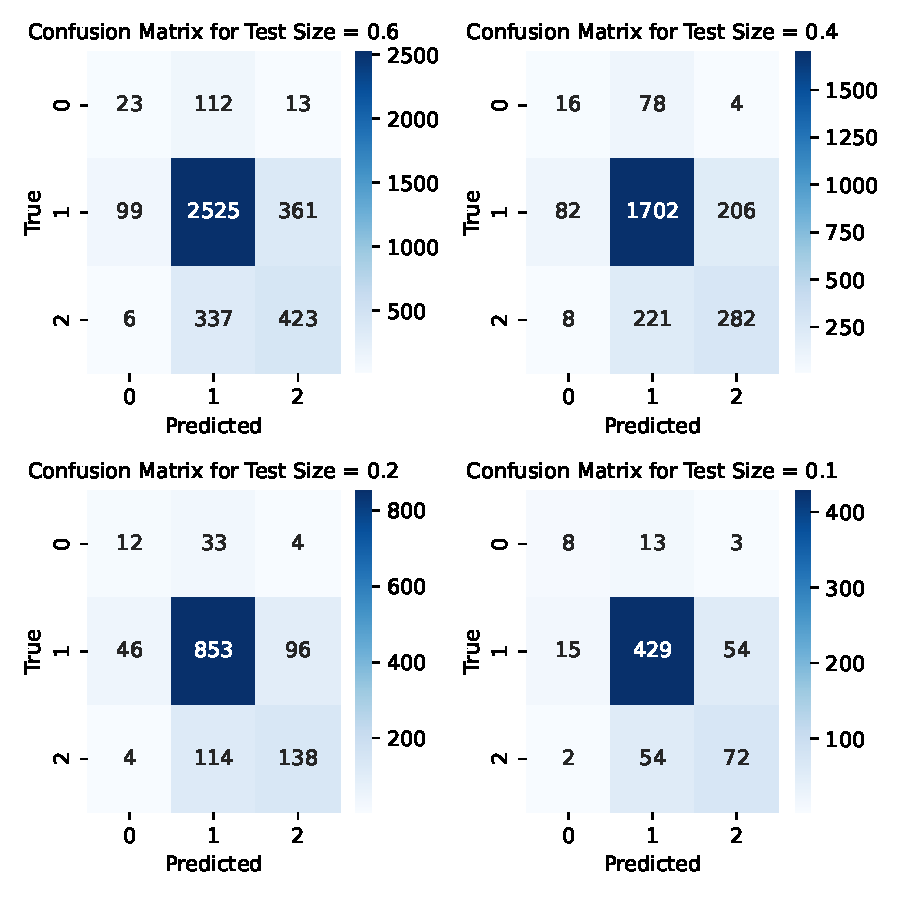
\includegraphics[width=.7\textwidth]{figures/wine_quality_confusion_matrices.pdf}
    \caption{Wine Quality dataset Confusion Matrices with different test sizes}
    \label{fig:wine_quality_confusion_matrices}
\end{figure}
% Confusion Matrix for Test Size = 0.6:
% [[  23  112   13]
%  [  99 2525  361]
%  [   6  337  423]]
% Confusion Matrix for Test Size = 0.4:
% [[  16   78    4]
%  [  82 1702  206]
%  [   8  221  282]]
% Confusion Matrix for Test Size = 0.2:
% [[ 12  33   4]
%  [ 46 853  96]
%  [  4 114 138]]
% Confusion Matrix for Test Size = 0.1:
% [[  8  13   3]
%  [ 15 429  54]
%  [  2  54  72]]

The confusion matrices in figure \ref{fig:wine_quality_confusion_matrices} show that the Decision Tree classifier performs well on the standard quality class but struggles with the low and high-quality classes. The classifier misclassifies many low-quality samples as standard quality and high-quality samples as standard quality. This behavior is expected due to the class imbalance in the dataset.

\subsection{Depth vs Accuracy evaluation}

The Decision Tree classifier's performance is evaluated by varying the maximum depth of the tree. The accuracy of the classifier is computed for different maximum depths using the \texttt{accuracy\_score} function from the \texttt{sklearn.metrics} module for the Decision Tree classifier with a test size of 20\%.

\begin{figure}[H]
    \centering
    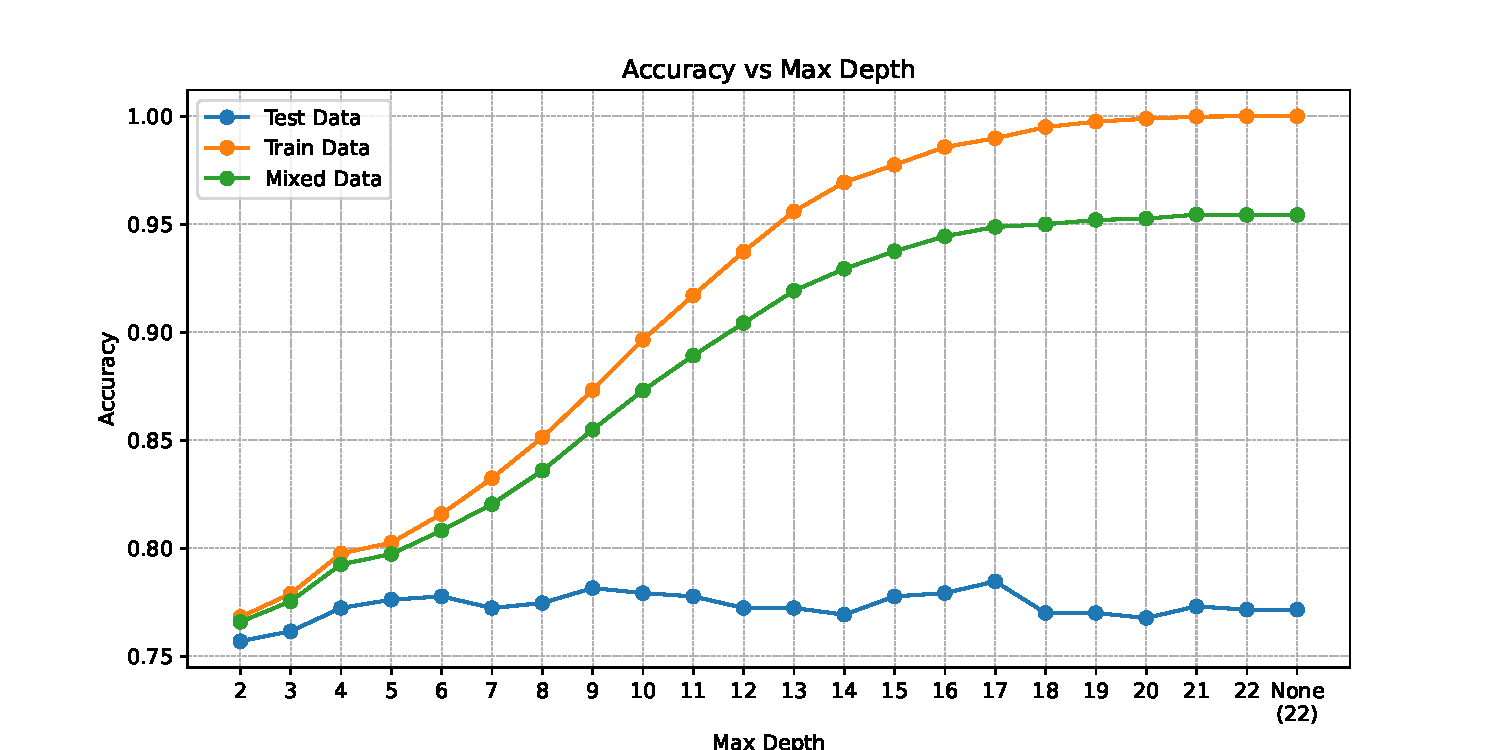
\includegraphics[width=\textwidth]{figures/wine_quality_accuracy_vs_max_depth.pdf}
    \caption{Breast Cancer Wisconsin dataset Depth vs Accuracy}
    \label{fig:wine_quality_accuracy_vs_max_depth}
\end{figure}

The plot in figure \ref{fig:wine_quality_accuracy_vs_max_depth} shows that the Decision Tree classifier achieves the highest accuracy on the test data when the maximum depth is around 17. The accuracy slightly fluctuates around 0.77 for all depths, indicating that the model's performance is relatively stable.



\newpage
\setcounter{section}{3}
\setcounter{subsection}{0}
\Section{Dataset 3: The UCI User Knowledge Modeling}

In this Section, we will present the classification results of the dataset that we used in our project, which is the UCI User Knowledge Modeling dataset \cite{user_knowledge_modeling}.

The User Knowledge Modeling dataset provides real-world data about students' knowledge status on the subject of Electrical DC Machines. The dataset was obtained as part of a Ph.D. thesis and has been analyzed to classify the knowledge levels of students based on various input features. The knowledge classes were determined in the thesis using a hybrid machine learning technique combining k-Nearest Neighbors (k-NN) with meta-heuristic exploration methods.

\subsubsection*{Dataset Characteristics}
\begin{itemize}
    \item \textbf{Type:} Multivariate
    \item \textbf{Subject Area:} Computer Science
    \item \textbf{Associated Tasks:} Classification, Clustering
    \item \textbf{Feature Type:} Integer
    \item \textbf{Number of Instances:} 403
    \item \textbf{Number of Features:} 5
    \item \textbf{Missing Values:} No
\end{itemize}

\subsubsection*{Dataset Insights}
\begin{itemize}
    \item \textbf{Objective:} To classify students' knowledge levels about Electrical DC Machines into predefined classes based on input features related to study habits and exam performance.
    \item \textbf{Classification Methodology:} The authors utilized an intuitive knowledge classifier, which combines k-Nearest Neighbor (k-NN) with meta-heuristic methods for classifying knowledge levels.
    \item \textbf{Class Distribution:} The dataset contains imbalanced classes:
    \begin{itemize}
        \item Very Low: 50 instances
        \item Low: 129 instances
        \item Middle: 122 instances
        \item High: 102 instances
    \end{itemize}
\end{itemize}

\subsubsection*{Feature Description}
\begin{itemize}
    \item \textbf{Input Variables:}
    \begin{enumerate}
        \item \textbf{STG:} The degree of study time for goal object materials.
        \item \textbf{SCG:} The degree of repetition of goal object materials.
        \item \textbf{STR:} The degree of study time for related objects with the goal object.
        \item \textbf{LPR:} The exam performance for related objects with the goal object.
        \item \textbf{PEG:} The exam performance for the goal objects.
    \end{enumerate}
    \item \textbf{Output Variable:}
    \begin{itemize}
        \item \textbf{UNS:} The knowledge level of the user, classified into four categories:
        \begin{enumerate}
            \item Very Low
            \item Low
            \item Middle
            \item High
        \end{enumerate}
    \end{itemize}
\end{itemize}

\subsection{Data preparation}

\subsubsection{Import the dataset}

The \href{https://archive.ics.uci.edu/}{UC Irvine Machine Learning Repository} allows for direct dataset import in Python using the \texttt{ucimlrepo} package. The package is included in the \texttt{requirements.txt} file. The following code demonstrates how to import the Wine Quality (id = 257) dataset using the \texttt{fetch\_ucirepo} function:

\lstset{style=code}
\begin{lstlisting}[language=Python]
from ucimlrepo import fetch_ucirepo 

breast_cancer_wisconsin_diagnostic = fetch_ucirepo(id=257) 
    
X = breast_cancer_wisconsin_diagnostic.data.features 
y = breast_cancer_wisconsin_diagnostic.data.targets 
\end{lstlisting}

\subsubsection{Splitting the dataset}

The dataset is split into training and testing sets using the \texttt{train\_test\_split} function from the \texttt{sklearn} library. 
The dataset is splitted into 4 sets of different test sizes: 60\%, 40\%, 20\%, and 10\% of the dataset in stratified fashion, using the random state of 22125 to ensure reproducibility.

\begin{figure}[H]
    \centering
    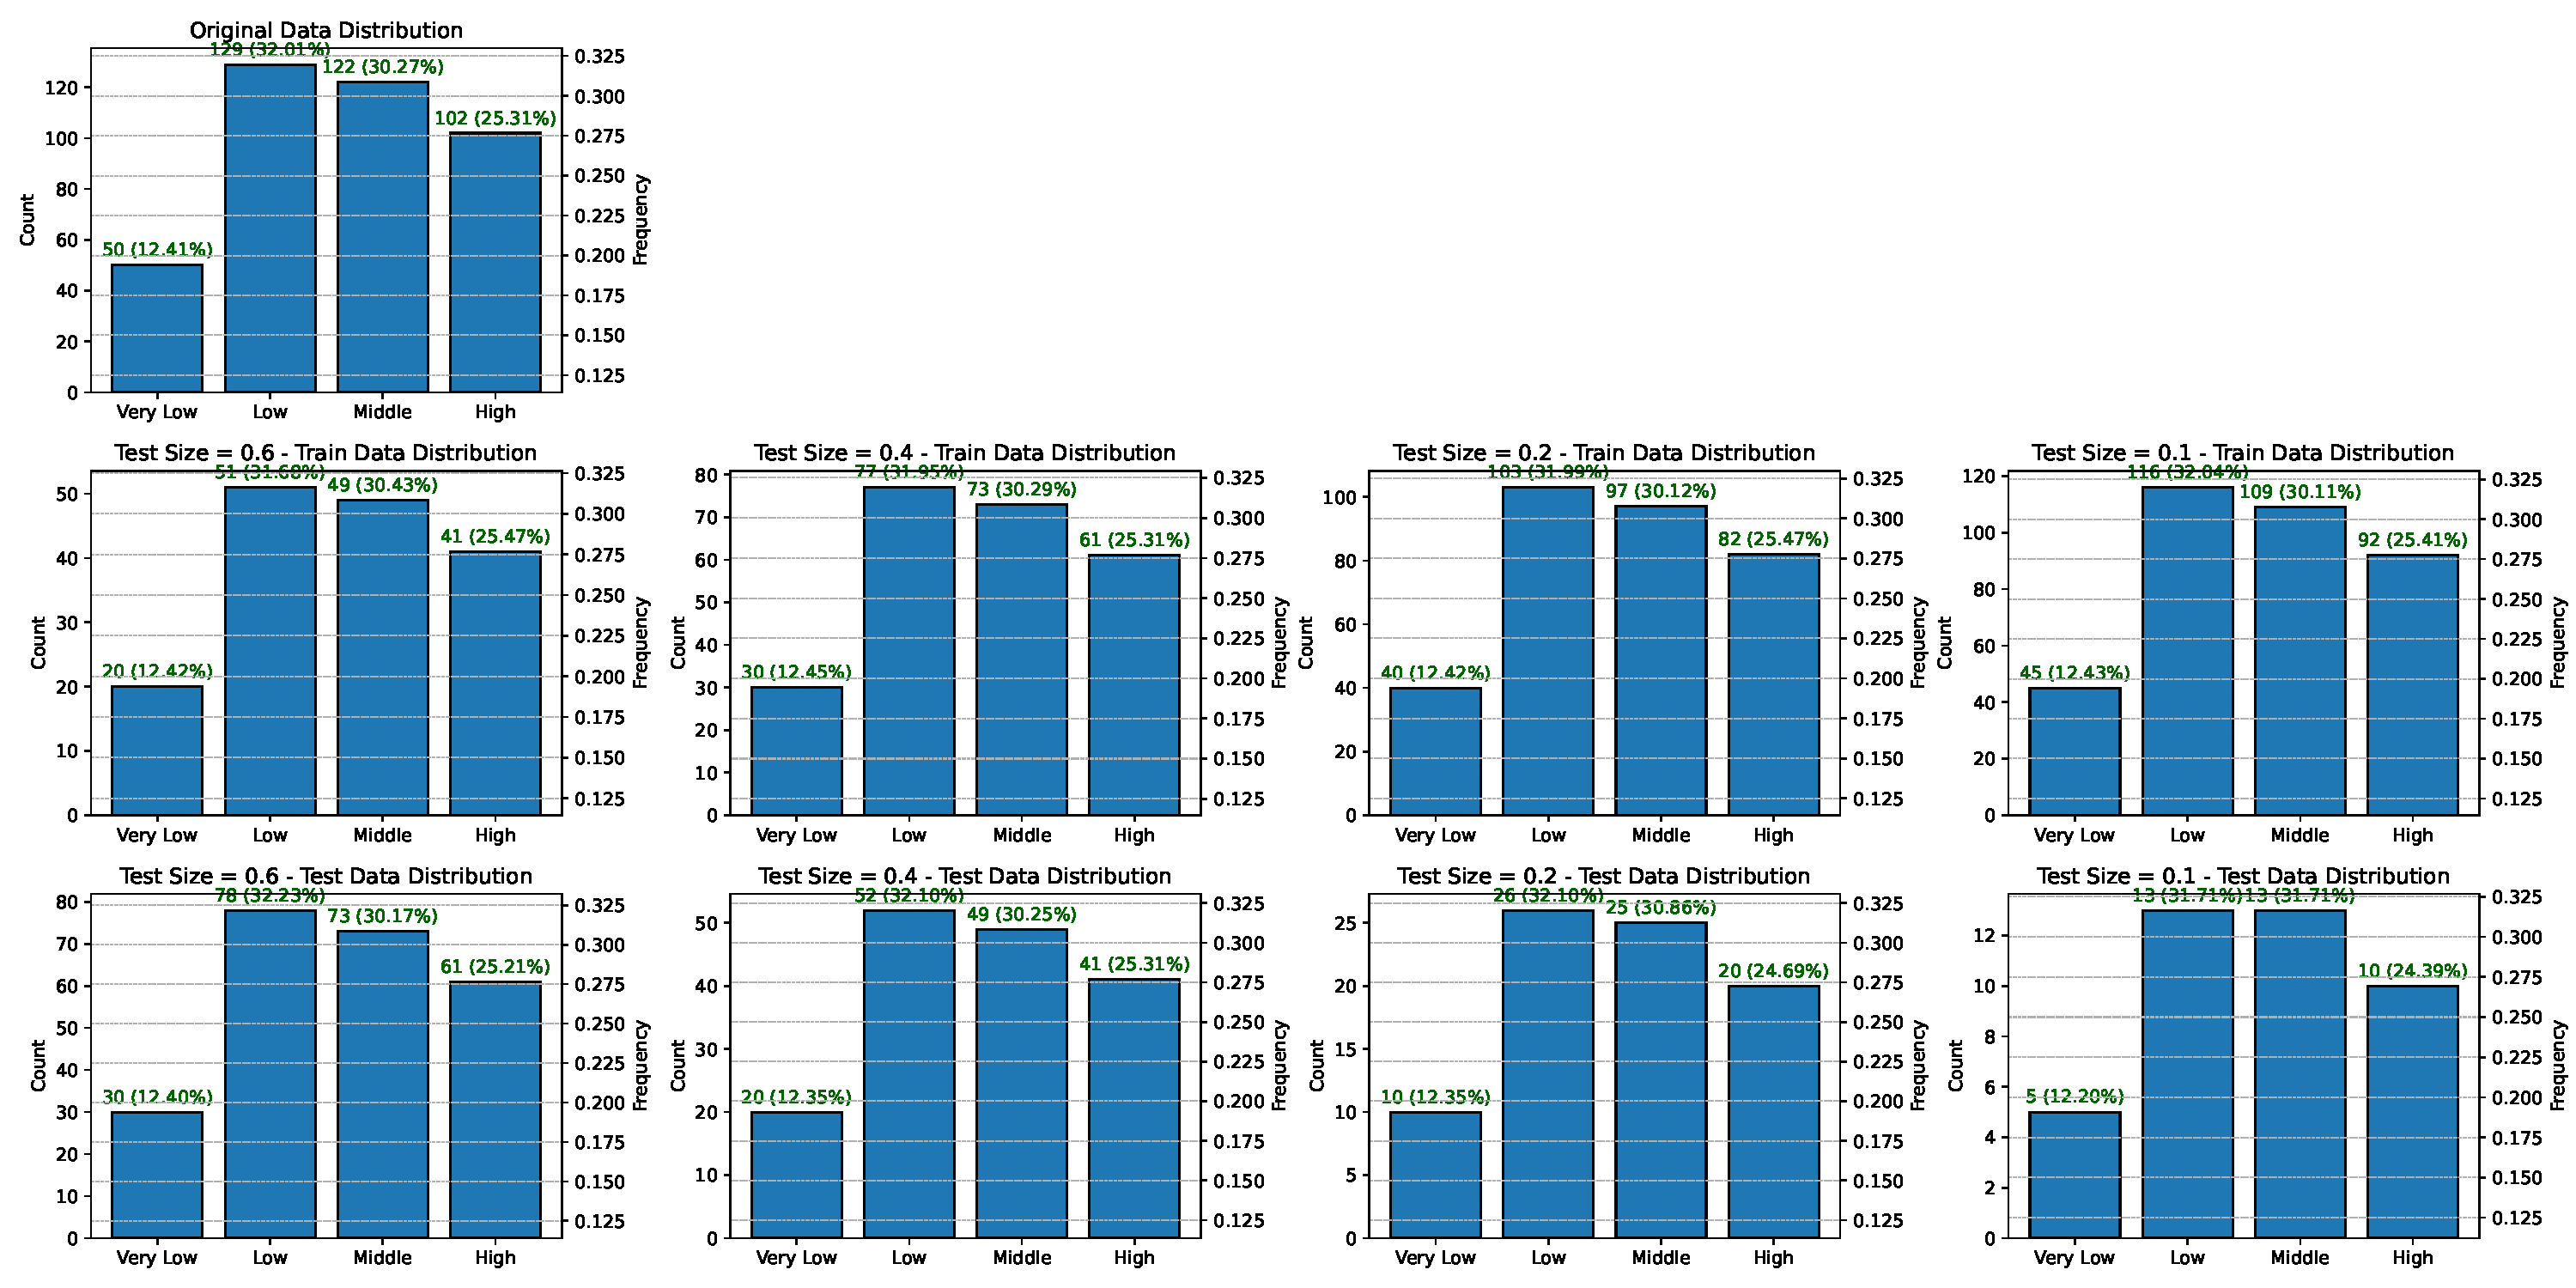
\includegraphics[width=\textwidth]{figures/user_knowledge_modeling_split.pdf}
    \caption{User Knowledge Modeling dataset splits}
    \label{fig:user_knowledge_modeling_split}
\end{figure}

As shown in figure \ref{fig:user_knowledge_modeling_split}, the distribution of the target class is preserved in all splits.

\subsection{Decision Tree classifier implementation}

Decision Tree classifiers are implemented using the \texttt{DecisionTreeClassifier} class from the \texttt{sklearn} library. 
To ensure reproducibility, the random state is set to 22125. 
We use the Entropy (information gain) criterion to split the nodes and set the maximum depth of the tree to None to allow the tree to grow until all leaves are pure.

\begin{figure}[H]
    \centering
    \includegraphics[width=\textwidth]{figures/user_knowledge_modeling_decision_trees.pdf}
    \caption{User Knowledge Modeling dataset Decision Trees with different test sizes}
    \label{fig:user_knowledge_modeling_decision_trees}
\end{figure}

The Decision Trees are visualized in figure \ref{fig:user_knowledge_modeling_decision_trees}. The trees grow deeper as the test size decreases, indicating that the model is more complex and overfits the training data when the test size is small.

The first node of the Decision Tree agrees on the feature \texttt{PEG} to split the dataset for all test sizes. This feature is likely the most discriminative for classifying the knowledge levels of students.

The first node's entropy is approximately 1.924 in all Decision Trees, indicating that the first split is not very informative. However, the Decision Tree classifier effectively splits the dataset into pure leaves with high information gain.

\subsection{Performance evaluation}

\subsubsection{Classification report}

The classification report provides a comprehensive evaluation of the Decision Tree classifier's performance using the \texttt{classification\_report} function from the \texttt{sklearn.metrics} module. The report includes the following metrics:
\begin{itemize}
    \item \textbf{Precision:} The ratio of true positive samples to the sum of true positive and false positive samples.
    \item \textbf{Recall:} The ratio of true positive samples to the sum of true positive and false negative samples.
    \item \textbf{F1-score:} The harmonic mean of precision and recall.
    \item \textbf{Support:} The number of samples in each class.
\end{itemize}

\textbf{Classification Report for Test Size = 0.6}

\begin{tabular}{lcccccc}
\hline
 & \textbf{Precision} & \textbf{Recall} & \textbf{F1-score} & \textbf{Support} \\
\hline
Very Low & 0.89 & 0.80 & 0.84 & 30 \\
Low & 0.87 & 0.88 & 0.88 & 78 \\
Middle & 0.88 & 0.84 & 0.86 & 73 \\
High & 0.88 & 0.97 & 0.92 & 61 \\
\hline
\textbf{Accuracy} & & & 0.88 & 242 \\
\textbf{Macro avg} & 0.88 & 0.87 & 0.88 & 242 \\
\textbf{Weighted avg} & 0.88 & 0.88 & 0.88 & 242 \\
\hline
\end{tabular}

\vspace{2em}

\textbf{Classification Report for Test Size = 0.4}

\begin{tabular}{lcccccc}
\hline
 & \textbf{Precision} & \textbf{Recall} & \textbf{F1-score} & \textbf{Support} \\
\hline
Very Low & 0.84 & 0.80 & 0.82 & 20 \\
Low & 0.88 & 0.88 & 0.88 & 52 \\
Middle & 0.94 & 0.92 & 0.93 & 49 \\
High & 0.95 & 1.00 & 0.98 & 41 \\
\hline
\textbf{Accuracy} & & & 0.91 & 162 \\
\textbf{Macro avg} & 0.90 & 0.90 & 0.90 & 162 \\
\textbf{Weighted avg} & 0.91 & 0.91 & 0.91 & 162 \\
\hline
\end{tabular}

\vspace{2em}

\textbf{Classification Report for Test Size = 0.2}

\begin{tabular}{lcccccc}
\hline
 & \textbf{Precision} & \textbf{Recall} & \textbf{F1-score} & \textbf{Support} \\
\hline
Very Low & 1.00 & 0.70 & 0.82 & 10 \\
Low & 0.81 & 1.00 & 0.90 & 26 \\
Middle & 1.00 & 0.80 & 0.89 & 25 \\
High & 0.91 & 1.00 & 0.95 & 20 \\
\hline
\textbf{Accuracy} & & & 0.90 & 81 \\
\textbf{Macro avg} & 0.89 & 0.88 & 0.93 & 81 \\
\textbf{Weighted avg} & 0.90 & 0.90 & 0.92 & 81 \\
\hline
\end{tabular}

\vspace{200em}

\textbf{Classification Report for Test Size = 0.1}

\begin{tabular}{lcccccc}
\hline
 & \textbf{Precision} & \textbf{Recall} & \textbf{F1-score} & \textbf{Support} \\
\hline
Very Low & 1.00 & 0.40 & 0.57 & 5 \\
Low & 0.68 & 1.00 & 0.81 & 13 \\
Middle & 1.00 & 0.62 & 0.76 & 13 \\
High & 0.83 & 1.00 & 0.91 & 10 \\
\hline
\textbf{Accuracy} & & & 0.80 & 41 \\
\textbf{Macro avg} & 0.76 & 0.75 & 0.88 & 41 \\
\textbf{Weighted avg} & 0.79 & 0.80 & 0.86 & 41 \\
\hline
\end{tabular}

The classification reports show that the Decision Tree classifier achieves high precision, recall, and F1-score for all classes in the test data. The model has an accuracy of approximately 0.88, 0.91, 0.90, and 0.80 for test sizes of 60\%, 40\%, 20\%, and 10\%, respectively. The model performs well in classifying the knowledge levels of students based on the input features.

\subsubsection{Confusion matrix}

The confusion matrix provides a visual representation of the Decision Tree classifier's performance using the \texttt{confusion\_matrix} function from the \texttt{sklearn.metrics} module. The matrix shows the number of true positive, false positive, true negative, and false negative samples for each class.

\begin{figure}[H]
    \centering
    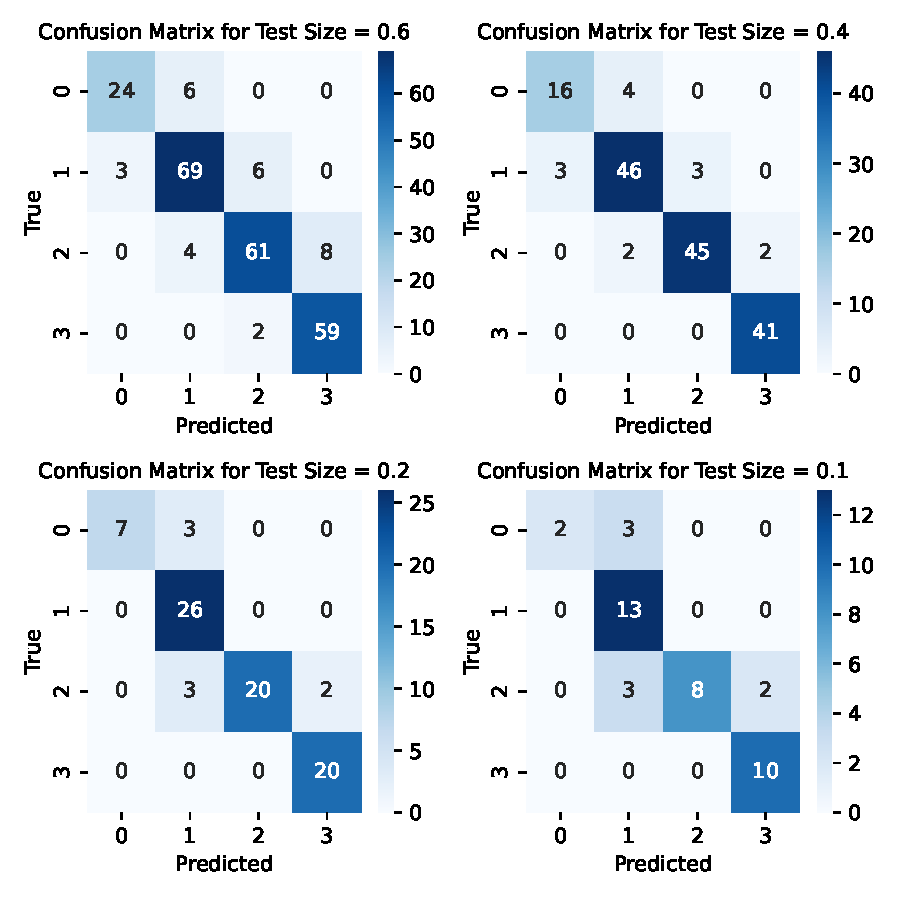
\includegraphics[width=.7\textwidth]{figures/user_knowledge_modeling_confusion_matrices.pdf}
    \caption{User Knowledge Modeling dataset Confusion Matrices with different test sizes}
    \label{fig:user_knowledge_modeling_confusion_matrices}
\end{figure}
% Confusion Matrix for Test Size = 0.6:
% [[24  6  0  0]
%  [ 3 69  6  0]
%  [ 0  4 61  8]
%  [ 0  0  2 59]]
% Confusion Matrix for Test Size = 0.4:
% [[16  4  0  0]
%  [ 3 46  3  0]
%  [ 0  2 45  2]
%  [ 0  0  0 41]]
% Confusion Matrix for Test Size = 0.2:
% [[ 7  3  0  0]
%  [ 0 26  0  0]
%  [ 0  3 20  2]
%  [ 0  0  0 20]]
% Confusion Matrix for Test Size = 0.1:
% [[ 2  3  0  0]
%  [ 0 13  0  0]
%  [ 0  3  8  2]
%  [ 0  0  0 10]]

The confusion matrices in figure \ref{fig:user_knowledge_modeling_confusion_matrices} show that the Decision Tree classifier correctly classifies most samples in the test data. The classifier has high true positive rates for all classes, indicating that the model effectively identifies the knowledge levels of students.

\subsection{Depth vs Accuracy evaluation}

The Decision Tree classifier's performance is evaluated by varying the maximum depth of the tree. The accuracy of the classifier is computed for different maximum depths using the \texttt{accuracy\_score} function from the \texttt{sklearn.metrics} module for the Decision Tree classifier with a test size of 20\%.

\begin{figure}[H]
    \centering
    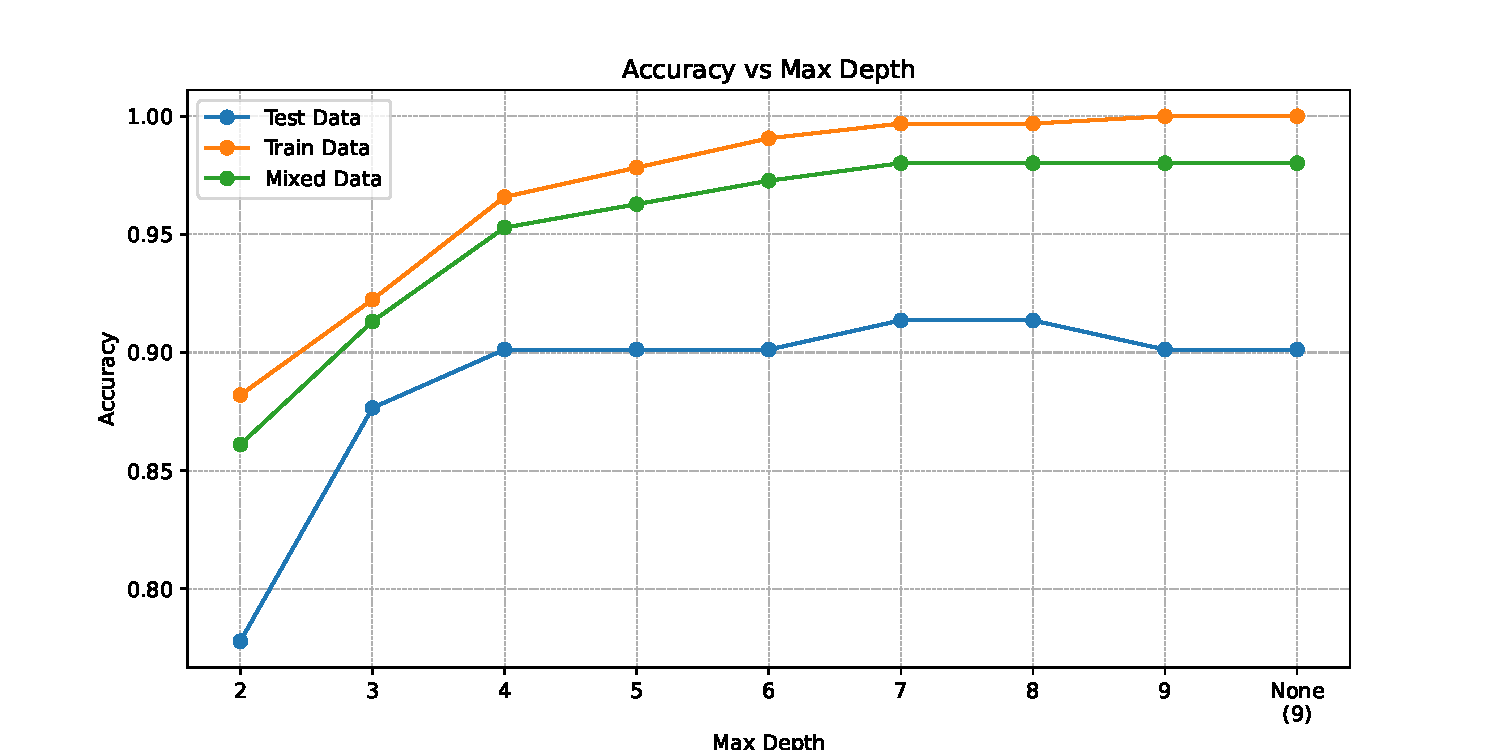
\includegraphics[width=\textwidth]{figures/user_knowledge_modeling_accuracy_vs_max_depth.pdf}
    \caption{User Knowledge Modeling dataset Depth vs Accuracy}
    \label{fig:user_knowledge_modeling_accuracy_vs_max_depth}
\end{figure}

The plot in figure \ref{fig:user_knowledge_modeling_accuracy_vs_max_depth} shows that the Decision Tree classifier achieves the highest accuracy on the test data when the maximum depth is around 7. The accuracy decreases slightly as the maximum depth increases beyond 7, indicating that the model starts to overfit the training data but still performs well on the test data.



\newpage
\Section{Comparison}

\begin{table}[H]
    \centering
    \begin{tabularx}{\textwidth}{|X|X|X|X|}
        \hline
        \makecell{\textbf{Criterion}} & 
        \makecell{\textbf{Breast Cancer} \\ \textbf{Wisconsin}} & 
        \makecell{\textbf{Wine} \\ \textbf{Quality}} & 
        \makecell{\textbf{User Knowledge} \\ \textbf{Modeling}} \\ \hline
        \textbf{Accuracy (80/20)} & 89\% & 77\% & 90\% \\ \hline
        \textbf{No. of Instances} & 569 & 4898 & 403 \\ \hline
        \textbf{No. of Features} & 30 & 11 & 5 \\ \hline
        \textbf{No. of Classes} & 2 & 3 & 4 \\ \hline
        \textbf{Imbalance} & Slight & Heavy & Balanced \\ \hline
        \textbf{Overfitting} & Yes & No & Slight \\ \hline
        \textbf{Complexity} & Medium & High & Medium \\ \hline
    \end{tabularx}
    \caption{Comparison of Decision Tree algorithm performance on different datasets}
\end{table}

\Section{Conclusion}

In this project, we implemented the Decision Tree algorithm using Python and the \texttt{scikit-learn} library. We evaluated the algorithm's performance on three different datasets from the UCI Machine Learning Repository.

We compared the algorithm's performance on the three datasets based on several criteria, including accuracy, number of instances, number of features, number of classes, imbalance, overfitting, and complexity.

The results show that the Decision Tree algorithm can achieve high accuracy on 2 out of 3 datasets. The algorithm performs well on the Breast Cancer Wisconsin dataset and the User Knowledge Modeling dataset, achieving an accuracy of 89\% and 90\%, respectively. However, the algorithm performs poorly on the Wine Quality dataset, achieving an accuracy of only 77\%. The poor performance on the Wine Quality dataset may be due to the dataset's complexity and the algorithm's inability to capture the underlying patterns in the data. 

The algorithm is simple to understand and interpret, making it an excellent choice for tasks that require transparency and interpretability.

\Section{Self-evaluation}

\Section{Contributions}

What the hell is this?

\newpage
\bibliographystyle{ieeetr}
\bibliography{references}
\addcontentsline{toc}{section}{References}

\end{document}